\documentclass[parskip=full]{scrartcl}

\usepackage[utf8]{inputenc}			% Umlaute, Sonderzeichen
\usepackage[ngerman]{babel}			% deutsche Sprache
\usepackage[tocfullflat]{tocstyle}			% Inhaltsverzeichnis
\usepackage{enumitem}				% Listen
\usepackage{graphicx}					% Grafiken
\usepackage{hyperref}					% Hyperlinks
\usepackage[nonumberlist]{glossaries}		% Glossar

% Hurenkinder und Schusterjungen verhindern
\clubpenalty10000
\widowpenalty10000
\displaywidowpenalty=10000

%\setcounter{tocdepth}{2}				% keine subsubsections im Inhaltsverzeichnis
\makenoidxglossaries

\newglossaryentry{bsp}{
	name=Beispiel,
	plural=Beispiele,
	description=Beispieleintrag }

\newglossaryentry{RasPi}{
	name=Raspberry Pi,
	description={Der Raspberry Pi ist ein Einplatinencomputer. In diesem Projekt dient der Raspberry Pi als Hardwareplattform, um unterschiedliche Sensoren zu verbinden und ihre Daten auszulesen.} }

\newglossaryentry{PhyPiDAQ}{
	name=PhyPiDAQ,
	description={Siehe Abschnitt 4.3 ,,PhyPiDAQ``} }

\newglossaryentry{Science Labs}{
	name=Science Labs,
	description={Ein Science Lab ist ein Arbeitsplatz, welcher Schülern ermöglicht wissenschaftliche Forschungen unter kontrollierten Bedingungen durchzuführen.} }

\newglossaryentry{Open-Source Projekt}{
	name=Open Source Projekt,
	description={Ein Open Source Projekt ist ein Projekt, wessen Quelltext und Dokumentationen von dritten angesehen, geändert und genutzt werden kann.} }

\newglossaryentry{OSL 2}{
	name=OSL 2,
	description={OSL 2 ist der Name eines Open-Source-Lehrsoftware-Labor, in welchem Studierende sich mit der Entwicklung von Open-Source-Software vertraut machen können.} }


\subject{Pflichtenheft}
\title{Visuelle Programmiersprache für den Physikunterricht zur Datenerfassung auf einem Raspberry Pi}
\subtitle{Version 0.2.0}
\author{David Gawron \and Stefan Geretschläger \and Leon Huck \and Jan Küblbeck \and Linus Ruhnke}
\date{\today}


\begin{document}

\maketitle

\newpage
\tableofcontents 					% generate pdf twice to update
\newpage

\section{Produktübersicht}



\section{Zielbestimmung}

Die Anwendung soll es Lehrern ermöglichen, Schülern ab der siebten Klasse Grundkenntnisse der digitalen Messwerterfassung in einer für Schüler interessante und motivierenden Weise näher zu bringen. 
Dabei werden aus didaktischer Sicht überflüssige technische Details wie z. B. die zum Auslesen der Sensoren notwendigen Protokolle vor dem Schüler verborgen.
Der Schüler wird so nicht überfordert, sondern soll ermutigt werden, selbstständig mit der Software umzugehen. 
Dabei kann er im spielerischen Umgang mit Versuchsaufbauten Prinzipien der digitalen Messtechnik wie z. B. Kaskadierung und natürlich auch das Grundprinzip von Ursache und Wirkung erfahren.

Es wird eine graphische Oberfläche angeboten, die es dem Schüler ermöglicht, allein per Drag and Drop eine Messanordnung zu erstellen. 
Überflüssige Details, die dahinter stecken, bleiben vor dem Schüler verborgen.
Die Anwendung motiviert den Schüler dazu, mit Sensoren, Transformationen und Darstellungen zu spielen und Dinge auszuprobieren. 
Dabei wird ihm durch eine intuitive Status- und Fehleranzeige gezeigt, ob seine Konstruktion funktioniert. 
Wenn nicht, dann zeigt sie ihm an, wo das Problem liegt und warum es nicht funktioniert. 
Eine lästige Fehlersuche soll dem Schüler weitestgehend erspart bleiben. 

Außerdem liefert die Anwendung dem Schüler zu den vorhandenen Bausteinen und zu der Anwendung allgemein die nötigen Informationen, die er für die Nutzung braucht. Dabei wird auf ein ausführliches Tutorial am Anfang verzichtet. Die Anwendung liefert die Informationen häppchenweise durch Informationsanzeigen an den jeweilig relevanten Stellen. Damit findet der Schüler die Hilfe, die er sucht, an der Stelle, an der er sie braucht.

Die Anwendung ermöglicht es dem Lehrer vor dem Unterricht, eine Reihe von Messversuchen teilweise oder ganz zu konfigurieren und zu speichern. Dabei kann er genau bestimmen, was er den Schülern zeigen will. Diese Konfigurationen kann er dann schnell und einfach im Unterricht zum Einsatz bringen. 

Weiter ermöglicht es die Anwendung, dass Schüler aus höheren Klassen mit mehr Details der digitalen Messwerterfassung zusammen gebracht werden. Diese nutzen keine oder nur eine abstrakt bzw. lückenhaft vorgefertigte Konfiguration. Sie können dann auch selbst einen Baustein modifizieren oder erstellen. Trotz des höheren Detailgrads bleibt die Anwendung übersichtlich und strukturiert. Damit bleiben auch komplexere Messversuche für den Schüler motivierend. 

Die Anwendung ist als Bindeglied zwischen \gls{PhyPiDAQ} und dem Nutzer zu verstehen. Sie ermöglicht dem Nutzer, über eine übersichtliche, strukturierte und intuitive GUI sowie über eine einfache Bedienung die Nutzung eines \gls{RasPi} mit \gls{PhyPiDAQ}. Dadurch soll dem Schüler digitale Messwerterfassung, Physik und auch Informatik in einer motivierenden Weise näher gebracht werden. Womöglich kann die Anwendung den Schüler auch für diese Themen begeistern.  

\subsection{Musskriterien}

\begin{itemize}

\item Datenhandhabung
\begin{itemize}

\item Der Benutzer kann Ergebnisse aus einer Messung speichern und laden.
\item Der Benutzer kann gleichzeitig Daten aus einer Messung darstellen und diese Daten auch weiter verwenden.
\item Der Benutzer kann eine Messkonfiguration speichern und laden.
\item Der Benutzer kann die Anwendung nutzen, ohne persönliche Daten preiszugeben.

\end{itemize}



\item Benutzbarkeit der GUI
\begin{itemize}

\item Die Anwendung reagiert auf Veränderungen so schnell, dass das Prinzip von Ursache und Wirkung intuitiv erfahren werden kann.
\item Der Benutzer kann Komponenten einer Messkonfiguration per Drag and Drop hinzufügen.
\item Der Benutzer kann Komponenten intuitiv mit einander verbinden.
\item Die Anwendung lässt sich mit dem Wissen eines Schülers aus der siebten Klasse bedienen.
\item Die Anwendung lässt sich auch mit einer rot-grün-Schwäche komplett nutzen.

\end{itemize}

\item Funktionen
\begin{itemize}

\item Die Anwendung erhält Daten durch den Raspberry Pi mit PhyPiDAQ oder aus einer Datei und kann diese dann transformieren und darstellen.
\item Die Anwendung enthält vorgefertigte Standardelemente, wie z.B. to do
\item Die Anwendung enthält vorgefertigte Standardkonfigurationen.

\end{itemize}

\item Information und Rückmeldung
\begin{itemize}

\item Ist ein verwendeter Sensor nicht angeschlossen oder fehlerhaft, meldet die Anwendung dies über eine Pop-Up-Nachricht.
\item Die Anwendung enthält Erklärungen und Informationen zu den einzelnen Komponenten, d.h. zu den Sensoren, Transformationen und Darstellungen.
\item Die Anwendung enthält Erklärungen und Informationen zu den GUI-Bereiche, d.h. zu dem Auswahlbereich der Komponenten, zu dem Messversuchsbereich und zu dem Anzeigebereich.
\item Falls nicht alle Kanäle verbunden sind, meldet die Anwendung dies dem Benutzer mit einer Fehlermeldung, falls dieser versucht die Messung zu starten. 

\end{itemize}

\item Sonstiges
\begin{itemize}

\item Die Anwendung kommuniziert mit den Nutzer auf deutsch.
\item Die Anwendung soll auf die Unterstützung neuer Sensoren erweiterbar sein.
\item Die Anwendung hält die Datenschutzrichtlinie "`to do"' ein.
\item Die Anwendung hält die Schulrichtlinie "`to do"' ein.

\end{itemize}

 \end{itemize}

\subsection{Sollkriterien}

\begin{itemize}

\item Die Anwendung soll auf die Erstellung eigener Transformationen erweiterbar sein.
\item Die Anwendung soll auf andere Sprachen erweiterbar sein.
\item Die Anwendung soll allein auf dem \gls{RasPi} laufen können.
\item Farbkodierung der GUI-Elemente
\item Einfache Erweiterbarkeit
\subitem Einheitliches Interface für Sensoren


 \end{itemize}

\subsection{Wunschkriterien}

\begin{itemize}

\item Übertragung der Messdaten über Netzwerkschnittstelle
\item Spiele, „nachmachen“ von vorgegebenen Messergebnissen
\item Ausführliche Beschreibung der physikalische Hintergründe

 \end{itemize}

\subsection{Abgrenzungskriterien}

\begin{itemize}

\item Unterschiedliche Benutzerkonten sind nicht zu implementieren
\item Personenbezogene Daten werden nicht gespeichert

 \end{itemize}

\section{Produkteinsatz}

\subsection{Anwendungsbereiche}

Die Anwendung ist für die Verwendung in Schulklassen ab der 7. bis zu 10. Klasse für Schüler und Lehrer im Physikunterricht konzipiert. Ebenfalls soll die Anwendung in Physikprojekten, sowie \gls{Science Labs} verwendet werden können. 
Als \gls{Open-Source Projekt} Im Rahmen des \gls{OSL 2} steht die Anwendung jedoch jedem Interessierten zur Verwendung und Weiterentwicklung zur Verfügung.


\subsection{Zielgruppe}

Die Zielgruppen sind hauptsächlich Schülerinnen und Schüler im Physikunterricht, welche die Anwendung verwenden, um erste eigene Messungen durchzuführen. Das Ziel ist es den Schülern erste Einblicke in Messtechniken und Zusammenhänge zwischen Ursache und Wirkung zu zeigen. 
Die Anwendung soll ebenfalls nicht nur von physikbegeisterten Schülern verwendet werden können, sondern auch für Schüler ohne ein großes Vorwissen in der Physik und Messtechniken eine interessante Plattform zu bieten, welche einfach zu verwenden ist.

\subsection{Betriebsbedingungen}

Die Anwendung läuft auf gewöhnlichen Schulcomputern, welche über eine USB-Schnittstelle mit einem RasPi verbunden sind, auf welchem das Programm \gls{PhyPiDAQ} läuft. Über das \gls{PhyPiDAQ} werden die an das RasPi angeschlossenen Messsensoren adressiert, welche die Messdaten wiederum über das RasPi an die am Computer gelaufende Anwendung schicken. 


\section{Produktumgebung}

Die Anwendung läuft auf einem Computer, die Messdaten werden über Messsensoren an einem \gls{RasPi} erfasst.

\subsection{Software}

Die Anwendung läuft auf Computern mit den Betriebssystemen Linux ab Kernel 7 und Microsoft Windows ab Windows 7 oder neuer. Die Anwendung muss auf dem Computer vollständig installiert sein. 

\subsection{Hardware}

Die Anwendung läuft auf gewöhnlichen Computern.
Auf dem per USB-Schnittstelle verbundenen \gls{RasPi} muss PhyPiDAQ installiert und verwendungsfähig sein.
Die an den Raspberry Pi angeschlossenen Messsensoren müssen richtig und sinnvoll angeschlossen sein.

\subsection{PhyPiDAQ}

Bei PhyPiDAQ\footnote{\url{https://github.com/GuenterQuast/PhyPiDAQ}} handelt es sich um eine Anwendung zur Datenerfassung und Analyse mit einem \gls{RasPi}. Diese ist nicht Bestandteil des Produktes, wird jedoch zur Datenerfassung und Datenverarbeitung und somit zur Funktionalität der Anwendung  benötigt. Das Programm, welches in der Programmiersprache python3 geschrieben ist bietet einfache und einheitliche Schnittstellen zur Verwendung der Messsensoren.


\section{Funktionale Anforderungen}


\subsection{GUI}

\begin{itemize}
\item[F010] Die Benutzer erreichen nach Öffnung der Anwendung direkt die GUI.
\item[F020] Der Benutzer öffnet durch den Optionen-Knopf die Einstellungen.
\item[F030] Der Benutzer kann durch den Datei-Knopf die Dateiverwaltung öffnen.
\item[F040] Der Benutzer kann durch den Hilfe-Knopf das Hilfe Fenster öffnen.
\end{itemize}

\subsubsection{Menüfeld}

\begin{itemize}
\item[F050] Der Benutzer öffnet durch den Sensoren-Knopf die Auswahl an Sensoren.
\item[F060] Der Benutzer öffnet durch den Verbindungen-Knopf die Auswahl an Verbindungen.
\item[F070] Der Benutzer öffnet durch den Darstellungen-Knopf die Auswahl an Darstellungen.
\item[F080] Der Benutzer erhält durch verschiedene Farben der Konfigurationsbausteine eine visuelle Repräsentationen ihrer Komplexität.
\end{itemize}

\subsubsection{Optional: Zusätzliche Funktionen im Menüfeld}

\begin{itemize}

\item[F090] Der Benutzer kann durch den Sensoren hinzufügen-Knopf weitere Sensoren hinzufügen.
\item[F100] Der Benutzer kann durch den Transformationen hinzufügen-Button weitere Transformationen hinzufügen.
\item[F110] Die in Transformationen in F100 sollen in eigenen Python-Skripten geschrieben werden.
\end{itemize}

\subsubsection{Konfigurationsfeld}

\begin{itemize}
\item[F120] Durch Drag und Drop kann der Benutzer Konfigurationsbausteine im Konfigurationsfeld platzieren.
\item[F130] Durch Betätigen des Messung starten-Knopf startet der Nutzer eine Messung.
\end{itemize}


\subsubsection{Darstellungsfenster}

\begin{itemize}
\item[F140] Das Darstellungsfenster ist bei der Initialisierung der Anwendung leer.
\item[F150] Durch die Benutzerkonfiguration im Konfigurationsfeld wird durch F090 automatisch die Darstellungsart im Darstellungsfenster geöffnet.
\end{itemize}



\subsection{Konfigurationserstellung}

\begin{itemize}

\item[F160] Über F030 kann der Benutzer gespeicherte Standartkonfigurationen öffnen oder alte Messwerte verwenden.
\item[F170] Durch F160 geladene Konfigurationen und Messdaten werden automatisch nach Format überprüft.
\item[F180] Aus F050 kann der Benutzer Sensoren durch Drag und Drop in das Konfigurationsfeld ziehen.
\item[F190] Die Anwendung sollte automatisch überprüfen, ob der ausgewählte Sensor richtig angeschlossen ist.
\item[F200] Die Anwendung gibt durch F190 automatisch eine visuelle Rückmeldung über die Farbe des Sensors und einer Pop-Up Benachrichtigung.
\item[F210] Aus F060 kann der Benutzer eine oder mehrere Verbindungen durch Drag und Drop in das Konfigurationsfeld ziehen.
\item[F220] Die ausgewählten Verknüpfungen kann der Benutzer mit einem ausgewählten Sensor verknüpfen.
\item[F230] Die Anwendung sollte automatisch überprüfen, ob die Verbindungen eine geeignete Kombination mit dem Sensor darstellt.
\item[F240] Aus F070 kann der Benutzer eine Darstellungsart per Drag und Drop in das Konfigurationsfeld zu ziehen.
\item[F250] Die Ausgewählte Darstellung kann der Benutzer mit einer Verbindung verknüpfen.
\item[F260] Die Anwendung sollte automatisch überprüfen, ob die gewählte Darstellungsart eine sinnvolle Repräsentation der Messdaten darstellt.
\item[F270] Über F030 kann der Benutzer seine eigene Konfiguration über einen Konfiguration speichern-Knopf speichern.
\item[F280] Bausteine die ein Benutzer nicht mehr in dem Konfigurationsfeld haben möchte können durch Drag und Drop in die Menüleiste wieder versteckt werden.

\end{itemize}

\subsubsection{Optional: Weiterentwicklung der Konfigurationserstellung}

\begin{itemize}

\item[F290] Die Anwendung besitzt einen Check-Knopf, welcher die Benutzerkonfiguriation auf Vollständigkeit und Richtigkeit
kontrolliert
\item[F300] Durch F290 wird durch visuelle Darstellung der Konfigurations dargestellt, ob sie verwendet werden kann.

\end{itemize}

\subsection{Messablauf}

\begin{itemize}

\item[F310] Der Nutzer kann in den Optionen, die Messlänge und die Wertebereiche festlegen.
\item[F320] Der Nutzer kann durch F130 die Messung nach der Benutzerkonfiguration starten.
\item[F330] Durch F320 wird automatisch mit der visuellen Darstellung der Messdaten begonnen.
\item[F340] Der Nutzer kann durch den Messung Messung löschen-Knopf eine durchgeführte Messung pausieren und die visuelle Darstellung auf den Ausgangszustand bringen.
\item[F350] Durch F340 wird nicht die Benutzerkonfiguration gelöscht.
\item[F360] Durch F340 muss der Benutzer erst die Messung starten um weiter zu messen.
\item[F370] Der Benutzer kann durch den Messung pausieren-Knopf die Messung pausieren.
\item[F380] Der Benutzer kann durch den Messung-fortsetzen-Knopf die Messung fortsetzen.
\item[F390] Der Benutzer kann eine Messung durch F380 nur fortsetzen, wenn sie zuvor durch F370 pausiert wurde.
\item[F400] Der Benutzer kann durch den Messdaten speichern-Knopf die gemessenen Daten speichern.
\item[F410] Der Benutzer kann durch den Graph speichern-Knopf den durch die Messung erzeugten Graphen speichern.
\item[F420] Bei F400 und F410 öffnet sich automatisch das Verzeichnis und der Nutzer muss einen eigenen Dateinamen eingeben und speichern. 



\end{itemize}

\subsection{Fehlermeldungen}

\begin{itemize}
\item[F430] Durch F170 geladene Konfigurationen und Messdaten werden automatisch nach Format überprüft und eine aussagekräftige Fehlermeldung zurückgegeben.
\item[F440] Durch F240 und F270 wird bei einer ungültigen Kombination von zwei Konfigurationsbausteinen eine aussagekräftige Fehlermeldung zurückgegeben
\item[F450] Die Anwendung sollte dem Benutzer automatisch durch Pop-Up Benachrichtigung darauf hinweisen, dass bei Betätigen des Messung löschen-Button oder bei Schließen der Anwendung die Messdaten ohne vorheriges Betätigen des Messdaten speichern-Button verloren gehen.
\item[F460] Die Anwendung sollte dem Benutzer eine aussagekräftige Fehlermeldung zurückgeben, falls es zu einem Datenabbruch der Messdaten kommt.

\end{itemize}



\subsection{Bedienungshilfen}

\begin{itemize}

\item[F470] Bei enthaltenen Konfigurationsbausteine sollen einen Information-Knopf besitzen, über welche der Benutzer Informationen und Hilfestellung bereitgestellt bekommt.
\item[F480] Über den Hilfe-Knopf erhält der Nutzer eine kurze Beschreibung zur Funktionalität der Anwendung.

\end{itemize}

\subsection{Sprache}

\begin{itemize}

\item[F490] Die Anwendung ist in deutscher Sprache.

\end{itemize}

\subsubsection{Optional: Internationalisierung}

\begin{itemize}

\item[F500] Die Anwendung stellt dem Benutzer weitere Sprachpakete für die GUI zur Verfügung.
\item[F510] Durch F020 ist die Sprache für den Nutzer änderbar.

\end{itemize}

\subsection{Sonstiges}

\begin{itemize}

\item[F520] Die in der Anwendung enthaltenen Farben sollten mit Rücksicht auf Benutzer mit Rot-Grün Schwäche oder Farbenblindheit ein barrierefreies Verwendung der Anwendung ermöglichen.

\end{itemize}

\subsubsection{Optional: Sonstiges}

\begin{itemize}

\item[F530] Durch F020 sollte der Benutzer die in der Anwendung verwendeten Farben ändern können.
\item[F540] Durch F020 sollte der Benutzer die in der Anwendung verwenden Buchstabengröße verändern können.

\end{itemize}


\section{Produktdaten}

Zu speichern sind ausschließlich:

\begin{itemize}

\item Konfigurationsdaten
\item Physikalische Messdaten

\end{itemize}

Es sollen keine benutzer- oder personenbezogenen Daten gespeichert werden.

\section{Nichtfunktionale Anforderungen}

\subsection{Produktleistungen}

\begin{itemize}

\item[NF010] Auslesen von Sensordaten innerhalb von (?) ms. //TODO PhyPiDAQ Abhängigkeit
\item[NF015] Alle (5?) ms können neue Daten angefordert werden.
\item[NF020] Verarbeitung ausgelesener Daten innerhalb von 10 ms.
\item[NF030] Bis zu drei Sensoren können zeitgleich verwendet werden.
\item[NF040] Bis zu (6?) Transformationen können hintereinander verbunden werden.
\item[NF050] Bis zu (3?) Senken können zeitgleich verwendet werden.

\end{itemize}

\subsection{Benutzbarkeit}

\begin{itemize}

\item[NF110] Die Benutzeroberfläche ist für Siebtklässler verständlich.
\item[NF120] Ungespeicherte Daten werden nicht ohne Warnung verworfen.
\item[NF130] Programmfehler werden dem Benutzer gegenüber klar kommuniziert.
\item[NF140] Schriftgröße von Text kann verändert werden.
\item[NF150] Farbschema von farbigen UI-Elementen ist veränderbar.

\end{itemize}

\subsection{Zuverlässigkeit}

\begin{itemize}

\item[NF210] Die Anwendung reagiert konsistent auf Eingaben.
\item[NF220] Korrekte Bedienung und Eingaben führen nicht zu unerwarteten Effekten.
\item[NF230] Unerwartete und fehlerhafte Eingaben führen nicht zum Systemabsturz.
\item[NF240] Verbindungsverlust von Sensoren führt nicht zum Systemabsturz.

\end{itemize}

\subsection{Sonstige}

\begin{itemize}

\item[NF310] Die Software ist vollständig quelloffen und frei.\footnote{\url{https://www.gnu.org/philosophy/free-sw.de.html}}
\item[NF320] Die Datenschutz-Grundverordnung wird nicht verletzt.

\end{itemize}

\section{Globale Testfälle und Testszenarien}

\begin{itemize} 

\item[T010] Erstmaliges Starten und Anpassen der Anwendung 
\begin{itemize}

\item []\textbf{Testziel} Teste das Verhalten der Anwendung beim ersten Aufruf und das Ausführen der Demo. Die Demo nutzt Daten aus einer Datei und benötigt keinen angeschlossenen \gls{RasPi}.

\item []\textbf{Vorbedingung} Die Anwendung ist installiert. Zu Sehen ist das offene Fenster des Desktops mit der Verknüpfung zur Anwendung.
\item [1.]\textbf{Aktion} Der Benutzer startet die Anwendung über die Verknüpfung.
\item []\textbf{Reaktion} Die Anwendung wird gestartet. Das Hauptfenster öffnet sich. Das Start-Infofenster öffnet sich.
\item [2.]\textbf{Aktion} Der Benutzer setzt den Haken bei "`dieses Fenster zukünftig nicht mehr anzeigen"'Knopf und drückt dann auf den "`Schließen"'Knopf des Start-Infofenster.
\item []\textbf{Reaktion} Das Start-Infofenster schließt sich. Die Start-Einstellung wird gespeichert. 
\item [3.]\textbf{Aktion} Der Benutzer drückt auf den "`Hilfe"'-Knopf in der Systemleiste.
\item []\textbf{Reaktion} Das Fenster zur Hilfe öffnet sich.
\item [4.]\textbf{Aktion} Der Benutzer drückt auf den "`Schließen"'-Knopf des Hilfefensters.
\item []\textbf{Reaktion} Das Fenster zur Hilft schließt sich.
\item [5.]\textbf{Aktion} Der Benutzer drückt auf den "`Laden"'-Knopf in der Systemleiste.
\item []\textbf{Reaktion} Das Fenster zum Laden einer Konfiguration öffnet sich. Dabei wird der voreingestellte default-Pfad geöffnet. 
\item [6.]\textbf{Aktion} Der Benutzer wählt die Demo-Datei in dem default-Pfad aus und drückt dann auf den "`Laden"'-Knopf. 
\item []\textbf{Reaktion} Die Anwendung lädt die Demo-Datei. Die geladene Demo-Konfiguration wird auf der Konfigurationsfläche angezeigt.
\item [7.]\textbf{Aktion} Der Lehrer drückt auf den "`Erstellen"'-Knopf.
\item []\textbf{Reaktion} Die Anwendung prüft, ob eine gültige Konfiguration vorliegt. Es liegt eine gültige Konfiguration vor. Die Anwendung zeigt den Konfigurationsstatus "`OK"' an.
\item [8.]\textbf{Aktion} Der Lehrer drückt auf den "`Starten"'-Knopf.
\item []\textbf{Reaktion} Die Anwendung verarbeitet die Daten der "`Sensoren"' und stellt die Ergebnisse dar.
\item [9.]\textbf{Aktion} Der Benutzer drückt auf den "`Stoppen"'-Knopf.
\item []\textbf{Reaktion} Die Ausführung der Messung wird angehalten. Die Darstellungen zeigen ihren Datensatz zum Zeitpunkt des Stoppens weiter an.
\item [10.]\textbf{Aktion} Der Benutzer drückt auf den auf das "`X"'-Symbol zum Schließen der Anwendung.
\item []\textbf{Reaktion} Es öffnet sich ein Fenster und weist den Benutzer darauf hin, dass nicht gespeicherte Daten und Veränderungen verloren gehen.
\item [11.]\textbf{Aktion} Der Benutzer drückt auf den "`Beenden"'-Knopf.
\item []\textbf{Reaktion} Die Anwendung schließt sich.

\item []\textbf{Nachbedingung} Die Anwendung ist beendet. Es ist kein Fenster ist mehr geöffnet. Es wird der Desktop angezeigt.
\item []\textbf{Ergebnis} to do

\item []\textbf{Abgedeckte Funktionale Anforderungen: to do}

\end{itemize}



\item[T020] Lehrer erstellt eine eigene Konfiguration für den Unterricht
\begin{itemize}

\item []\textbf{Testziel} Teste eine typische Verwendung der Software anhand des gegebenen Szenarios. Dabei wird das Erstellen, Verändern und Speichern einer Konfiguration getestet.

\item []\textbf{Vorbedingung} Die Anwendung ist gestartet und es liegt keine Konfiguration vor. Die Anwendung hat Zugriff auf einen laufenden RaspberryPi mit PhiPiDAQ. Die Sensoren die verwendet werden sollen sind ordnungsgemäß angeschlossen.

\item [1.]\textbf{Aktion} Der Lehrer zieht Sensor S1 in die Konfigurationsfläche. 
\item []\textbf{Reaktion} Die Anwendung prüft, ob Sensor S1 angeschlossen ist. Danach wird das Icon von Sensor S1 an der gewählten Stelle erstellt. Dabei werden Defaultwerte eingestellt.
\item [2.]\textbf{Aktion} Der Lehrer ruft die Optionen des Sensors auf(Rechtsklick Icon, dann Optionen).
\item []\textbf{Reaktion} Die Anwendung ruft das Fenster für die Optionen von Sensor S1 auf.
\item [3.]\textbf{Aktion} Der Lehrer setzt Werte im gültigen Bereich ein und drückt auf den "`Speichern"'-Knopf.
\item []\textbf{Reaktion} Die Einstellungen werden gespeichert und das Optionsfenster wird geschlossen.
\item [4.]\textbf{Aktion} Der Lehrer zieht die Transformation T in die Konfigurationsfläche.
\item []\textbf{Reaktion} Das Icon der Transformation T wird in der Konfigurationsfläche erstellt. Die Werte werden auf default eingestellt.
\item [5.]\textbf{Aktion} Der Lehrer ruft die Optionen von Transformation T auf.
\item []\textbf{Reaktion} Das Optionsfenster von Transformation T öffnet sich.
\item [6.]\textbf{Aktion} Der Lehrer stellt die Werte der Transformation im gültigen Bereich ein und drückt auf den "`Speichern"'-Knopf.
\item []\textbf{Reaktion} Die Werte werden gespeichert und das Optionsfenster wird geschlossen.
\item [7.]\textbf{Aktion}  Der Lehrer drückt auf den "`Optionen"'-Knopf der Konfiguration.
\item []\textbf{Reaktion} Das Optionsfenster für die Konfiguration öffnet sich.
\item [8.]\textbf{Aktion} Der Lehrer gibt verändert die Defaultwerte der Konfiguration und drückt auf den "`Speichern"'-Knopf.
\item []\textbf{Reaktion} Die Werte werden gespeichert und das Optionsfenster schließt sich.
\item [9.]\textbf{Aktion} Der Lehrer drückt auf den "`Konfiguration Speichern"'-Knopf
\item []\textbf{Reaktion} Die Anwendung öffnet das Fenster zum speichern einer Konfiguration.
\item [10.]\textbf{Aktion} Der Lehrer wählt einen gültigen Pfad, gibt einen gültigen Namen ein und drückt danach auf den "`Speichern"'-Knopf.
\item []\textbf{Reaktion} Die Anwendung erstellt eine Konfiguration-Datei mit entsprechendem Namen am entsprechenden Ort. Das Fenster zum Speichern einer Konfiguration wird geschlossen.


\item []\textbf{Nachbedingung} Die Anwendung ist geöffnet. In der Konfigurationsfläche ist Sensor S1 und Transformation T zu sehen. 
\item []\textbf{Ergebnis} Diese Konfiguration ist als Datei an dem gewählten Ort gespeichert.

\item []\textbf{Abgedeckte Funktionale Anforderungen: to do}

\end{itemize}

\item[T030] Schüler der siebten Klasse bearbeitet eine Aufgabe
\begin{itemize}

\item []\textbf{Testziel} Es soll getestet werden wie ein Schüler der siebten Klasse mit der Anwendung umgeht, während er eine Aufgabe des Lehrer bearbeitet. Dabei ist schon die Konfiguration aus T020 geladen. Diese enthält Sensor S1 und Transformation T.

\item []\textbf{Vorbedingung} Die Anwendung ist gestartet und es liegt eine vom Lehrer erstellte Konfiguration vor. Die Konfiguration enthält Sensor S1 und Transformation A. Die Anwendung hat Zugriff auf einen laufenden Raspberry Pi mit PhyPiDAQ. Die Sensoren S1 und S2 sind ordnungsgemäß angeschlossen.
\item [1.]\textbf{Aktion} Der Schüler drückt auf das "`?"'-Icon neben Sensor S1.
\item []\textbf{Reaktion} Es öffnet sich ein Infofenster zum Sensor S1.
\item [2.]\textbf{Aktion} Der Schüler drückt auf das "`?"'-Icon neben Transformation A.

\item []\textbf{Reaktion} to do: schließt sich Infofenster zu Sensor S1 automatisch oder bleibt es offen bis Schüler es schließt ?

\item [3.]\textbf{Aktion} Der Schüler drückt auf den "`Start"'-Knopf.
\item []\textbf{Reaktion} Ein Fenster öffnet sich und teilt dem Schüler mit, dass eine Konfiguration zunächst erstellt werden muss.
\item [4.]\textbf{Aktion} Der Schüler drückt auf den "`OK"'-Knopf.
\item []\textbf{Reaktion} Das Infofenster zum starten ohne erstellen wird geschlossen.
\item [5.]\textbf{Aktion} Der Schüler drückt auf den "`Erstellen"'-Knopf.
\item []\textbf{Reaktion} Die Anwendung prüft, ob die vorliegende Konfiguration gültig ist. Sie ist ungültig. Es wird ein Fenster geöffnet mit der Meldung, dass keine gültige Konfiguration vorliegt. Es verlinkt zum Hilfemenü.
\item [6.]\textbf{Aktion} Der Schüler drückt auf die Verlinkung zum Hilfsmenü.
\item []\textbf{Reaktion} Das Fenster zum Hilfsmenü öffnet sich. (TO DO wird Fehlermeldung geschlossen?)
\item [7.]\textbf{Aktion} Der Schüler drückt auf den "`X"'-Knopf des Hilfsmenüfensters. 
\item []\textbf{Reaktion} Das Hilfsmenüfenster wird geschlossen.
\item [8.]\textbf{Aktion} Der Schüler zieht die Darstellung D in die Konfigurationsfläche.
\item []\textbf{Reaktion} Ein Icon der Darstellung D wird erstellt. Es werden Defaultwerte geladen.
\item [9.]\textbf{Aktion} Der Schüler drückt auf das "`?"'-Icon der Darstellung.
\item []\textbf{Reaktion} Das Infofenster zu Darstellung D öffnet sich.
\item [10.]\textbf{Aktion} Der Schüler schließt das Infofenster.
\item []\textbf{Reaktion} Das Infofenster zu Darstellung D wird geschlossen.
\item [11.]\textbf{Aktion} Der Schüler drückt auf den Kanal von Darstellung D und danach auf den linken Kanal von Transformation T.
\item []\textbf{Reaktion} Eine Verbindung zwischen den beiden Kanälen wird erstellt.
\item [12.]\textbf{Aktion} Der Schüler drückt auf den oberen rechten Kanal von Transformation T und danach auf den Kanal von Sensor S1.
\item []\textbf{Reaktion} Eine Verbindung zwischen den beiden Kanälen wird erstellt.
\item [13.]\textbf{Aktion} Der Schüler zieht Sensor S2 in die Konfigurationsfläche.
\item []\textbf{Reaktion} Das Icon zu Sensor S2 wird erstellt.
\item [14.]\textbf{Aktion} Der Schüler ruft die Optionen von Sensor S2 auf.
\item []\textbf{Reaktion} Das Optionsfenster von Sensor S2 wird geöffnet.
\item [15.]\textbf{Aktion} Der Schüler gibt die vom Lehrer vorgegebenen Werte ein und drückt auf den "`Speichern"'-Knopf.
\item []\textbf{Reaktion} Die Werte werden gespeichert und das Optionsfenster von Sensor S2 wird geschlossen.
\item [16.]\textbf{Aktion} Der Schüler drückt auf den Kanal von S2 und danach auf den letzten offenen Kanal von Transformation T.
\item []\textbf{Reaktion} Eine Verbindung zwischen Sensors S2 und Transformation T wird erstellt.
\item [17.]\textbf{Aktion} Der Schüler drückt auf den "`Erstellen"'-Knopf.
\item []\textbf{Reaktion} Die Anwendung prüft, ob eine gültige Konfiguration vorliegt. Es liege eine gültige vor. Die Anwendung zeigt den Konfigurationsstatus "`OK"' an. Dabei wird durch die Voreinstellung der Lehrers aus T020 Aktion 8 und 9 der Messzeitraum auf 10 Sekunden gesetzt.
\item [18.]\textbf{Aktion} Der Schüler drückt auf "`Starten"'.
\item []\textbf{Reaktion} Die Anwendung holt für 10 Sekunden Daten aus den beiden Sensoren, transformiert diese und stellt sie in Darstellung D dar. Nach der Messung stoppt die Anwendung automatisch. Die Darstellung D bleibt erhalten.
\item [19.]\textbf{Aktion} Der Schüler drückt auf den Knopf "`Speichern"' bei der Darstellung.
\item []\textbf{Reaktion} Ein Fenster zum Speichern des Graphen öffnet sich.
\item [20.]\textbf{Aktion} Der Schüler wählt einen Pfad und gibt einen Namen ein und drückt dann auf den "`Speichern"'-Knopf.
\item []\textbf{Reaktion} Der Graph wird am entsprechenden Ort gespeichert und das Fenster zum Speichern wird geschlossen.
\item [21.]\textbf{Aktion} Der Schüler drückt auf den Knopf "`Messwerte speichern"'.
\item []\textbf{Reaktion} Ein Fenster öffnet sich zum Speichern der Messwerte.
\item [22.]\textbf{Aktion} Der Schüler wählt die Darstellungsform "`Tabelle"', den Pfad, den Namen und drückt auf den "`Speichern"'-Knopf.
\item []\textbf{Reaktion} Die Messwerte werden als Tabelle mit entsprechendem Namen am entsprechenden Ort gespeichert. Das Fenster zum Speichern schließt sich.
\item [23.]\textbf{Aktion} Der Schüler drückt auf den "`Speichern"'-Knopf der Konfiguration. 
\item []\textbf{Reaktion} Die Anwendung öffnet das Fenster zum Speichern einer Konfiguration.
\item [24.]\textbf{Aktion} Der Schüler wählt dort Name und Pfad aus und drückt auf den "`Speichern"'-Knopf.
\item []\textbf{Reaktion} Die Konfiguration wird entsprechend gespeichert. Das Fenster zum Speichern einer Konfiguration wird geschlossen.

\item []\textbf{Nachbedingung} Die Anwendung ist geöffnet. Nur das Hauptfenster ist offen. In der Konfigurationsfläche ist die vollständige Konfiguration zu sehen. Die Messung wurde abgeschlossen und die Darstellungen sind zu sehen.
\item []\textbf{Ergebnis} Die Konfiguration, die Messwerte sowie der Graph der Messwerte sind als Dateien gespeichert.

\item []\textbf{Abgedeckte Funktionale Anforderungen: TO DO}

\end{itemize}

\item[T040] Umgang mit destruktivem Benutzer
\begin{itemize}

\item []\textbf{Testziel} Teste den Umgang mit einem Benutzer, der versucht alle Grenzen der Anwendung und alle Fehlermeldungen zu finden.

\item []\textbf{Vorbedingung} Geöffnete Anwendung ohne angeschlossenem RaspberryPi und damit mit keinem gültigen Sensor.
\item [1.]\textbf{Aktion} Der Benutzer zieht Sensor S3 in die Konfigurationsfläche hinein.
\item []\textbf{Reaktion} Die Anwendung prüft ob der Sensor S3 angeschlossen ist. Er ist es nicht. Die Anwendung erstellt kein Icon, sondern öffnet eine Fehlermeldung, dass Sensor S3 nicht gefunden wurde.
\item [2.]\textbf{Aktion} Der Benutzer schließt die Meldung. Danach öffnet er über die Systemleiste das Menü um eine Datei als Sensor zu Initialisieren.
\item []\textbf{Reaktion} Die Fehlermeldung wird geschlossen. Das Menü zum Initialisieren einer Datei als Sensor wird geöffnet.
\item [3.]\textbf{Aktion} Der Benutzer wählt eine Datei mit ungültigem Format aus und drückt auf den "`Öffnen"'Knopf.
\item []\textbf{Reaktion} Die Anwendung prüft ob die Datei ein gültiges Format hat. Sie hat es nicht. Die Anwendung zeigt eine Fehlermeldung an, dass die gewählte Datei ein ungültiges Format hat.
\item [4.]\textbf{Aktion} Der Benutzer schließt die Fehlermeldung und wählt eine gültige Datei.
\item []\textbf{Reaktion} Die Anwendung prüft das Format, erkennt es als gültig und erstellt den Sensor S91. Das Fenster zum laden einer Datei wird geschlossen.
\item [5.]\textbf{Aktion} Der Benutzer lädt eine weitere gültige Datei als Sensor S92.
\item []\textbf{Reaktion} Die Anwendung öffnet das Ladefenster, prüft das Format der gewählten Datei, erkennt sie als gültig an und erstellt Sensor S92. Dann wird das Fenster zum Laden einer Datei geschlossen. 
\item [6.]\textbf{Aktion} Der Benutzer zieht erst Sensor S91 und dann Sensor S92 in die Konfigurationsfläche.
\item []\textbf{Reaktion} Die Anwendung prüft, ob Sensor S91 und S92 angeschlossen sind. Das sind sie, da sie aus gültigen Dateien stammen. Dann erstellt die Anwendung die entsprechenden Icons an den entsprechenden Stellen.
\item [7.]\textbf{Aktion} Der Benutzer drückt auf den Kanal von S91 und danach auf den Kanal von S92.
\item []\textbf{Reaktion} Die Anwendung erkennt, dass beide Kanäle von Sensoren stammen. Sie erstellt keine Verbindung und zeigt die Fehlermeldung an, dass zwischen zwei Sensoren keine Verbindung erstellt werden kann.
\item [.]\textbf{Aktion} Der Benutzer schließt die Fehlermeldung und zieht Transformation T1 in die Konfigurationsfläche. Dabei hat T1 zwei Eingangskanäle und einen Ausgangskanal.
\item []\textbf{Reaktion} Die Anwendung schließt die Fehlermeldung. Danach erstellt sie das Icon von T1 an der entsprechenden Stelle mit Defaultwerten.
\item [8.]\textbf{Aktion} Der Benutzer klickt auf den oberen Eingangskanal und danach auf den unteren Eingangskanal.
\item []\textbf{Reaktion} Die Anwendung erkennt, dass zwei Eingangskanäle verbunden werden sollen. Sie verbindet sie nicht, sondern zeigt die Fehlermeldung an, dass zwei Eingangskanäle einer Transformation nicht direkt verbunden werden können.
\item [9.]\textbf{Aktion} TO DO weitere Fehlerfälle
\item []\textbf{Reaktion}
\item [.]\textbf{Aktion} 
\item []\textbf{Reaktion}
\item [.]\textbf{Aktion} 
\item []\textbf{Reaktion}

\item []\textbf{Nachbedingung} TO DO
\item []\textbf{Ergebnis} TO DO

\item []\textbf{Abgedeckte Funktionale Anforderungen:} TO DO

\end{itemize}


\end{itemize}

\section{Systemmodelle}

\section{Benutzungsoberfläche}

\subsection{Ziel der Benutzeroberfläche}

Das Ziel der Benutzeroberfläche ist es dem Anwender eine intuitive Benutzung des Programmes zu ermöglichen. Da das Programm im Schulbetrieb eingesetzt werden soll ist eine gute Verständlichkeit wichtig. So soll auch eine lange Einarbeitungszeit für den Anwender vermieden werden. Dabei soll keine Funktionalität verloren gehen.

\subsection{Generell}

Um die Ziele zu erfüllen wird das Programm über eine Grafische Benutzeroberfläche (kurz "GUI") bedient. Der Anwender soll in der Lage sein bereits vorhandene Computer und Mobile-Device Kenntnisse zu nutzen.

\subsection{Eingabegeäte}

Die GUI ist überwiegend für die Bedienung durch die Maus ausgelegt. Dabei werden überwiegend folgende Aktionen verwendet:

\begin{itemize} 
	\item Click \newline Der linke Mausclick.
	\item Drag-And-Drop \newline Das Verschieben von Elementen durch das festhalten und anschließende loslassen der linken Maustaste.
\end{itemize}

Eine Tastatur wird benötigt um weitergehende Einstellungen, wie etwa das anpassen einer Option, zu ermöglichen.



\subsection{Überblick}

\begin{figure}[h]
	\begin{center}
		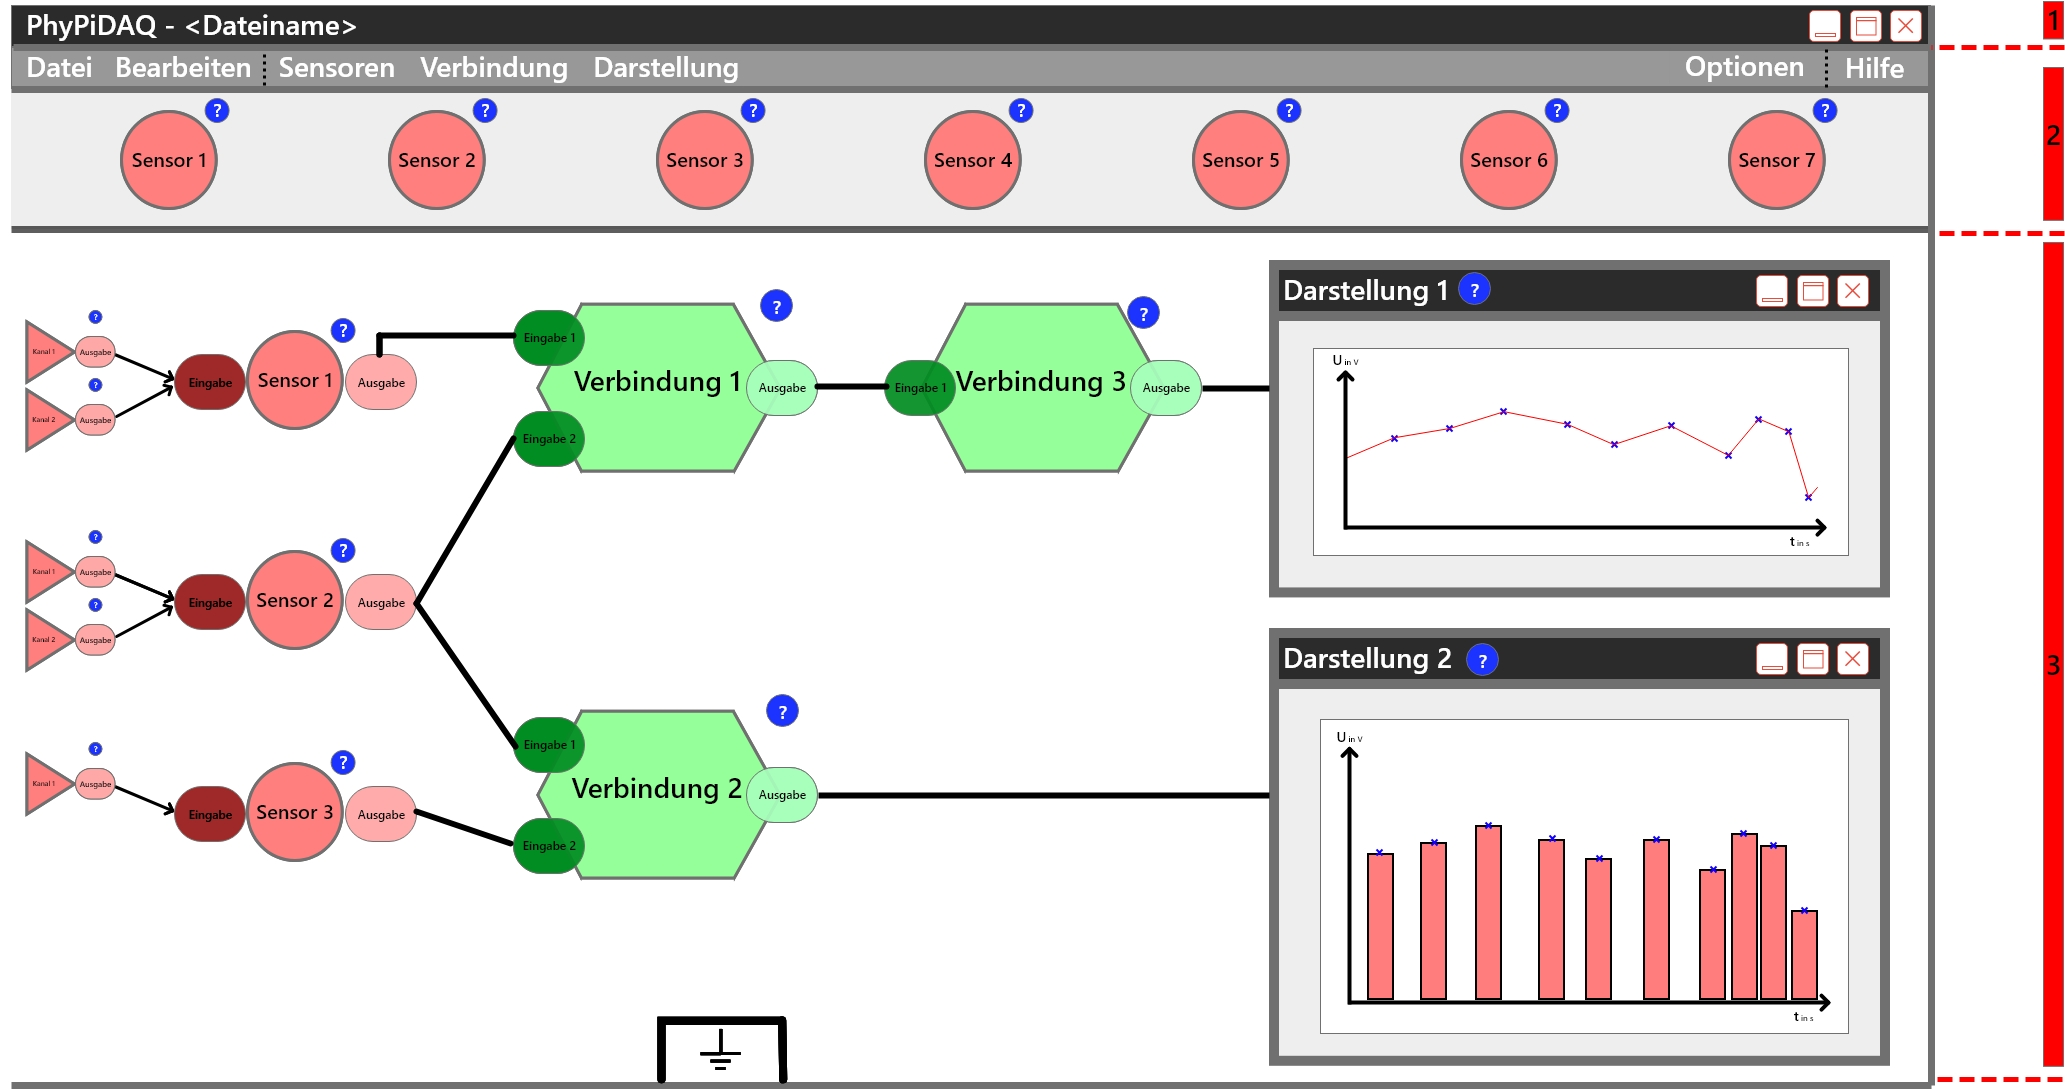
\includegraphics[width = 12cm]{Grafik/GUI-mit-Segmenten.jpg}
		\caption{Der Grundlegende Aufbau der Hauptbenutzeroberfläche}
		\label{GUI_Grundlage}
	\end{center}
\end{figure}

Abbildung 1 zeigt den Aufbau der Grafischen Benutzeroberfläche. Dabei geben die Zahlen in den roten Kästchen, rechts von dem Hauptfenster, die logische Unterteilung an.

Die zu dem jeweiligen Teil gehörenden Elemente sollen im folgenden erklärt werden.

\subsection{Die einzelnen Teile}

\subsubsection{Systemmenüleiste}

\begin{tabular}[t]{p{1cm} p{10cm}}
	\vspace{0cm}
\includegraphics[width = 1 cm]{Grafik/PhyPiDAQ.jpg} & Der Name des Programmes wird hier angezeigt. Rechts daneben steht, sofern vorhanden, der Name der Datei, die gerade geöffnet ist.\newline\\
	\vspace{0cm}
\includegraphics[width = 1 cm]{Grafik/Maximieren.jpg} & Das ''Maximieren''-Symbol vergrößert das Programmfenster auf die maximale Größe. Die Größe ist von der Benutzungsumgebung abhängig.\newline\\
	\vspace{0cm}
\includegraphics[width = 1 cm]{Grafik/Minimieren.jpg} & Das ''Minimieren''-Symbol blendet das Programmfenster aus. Es ist weiterhin geöffnet und wieder aufrufbar. \\
	\vspace{0cm}
\includegraphics[width = 1 cm]{Grafik/Schliessen.jpg} & Das ''Schließen''-Symbol beendet die Anwendung. Vor dem Beenden findet eine Abfrage statt, ob der Anwender eventuell vorgenommene Änderungen speichern möchte.\newline\\
\end{tabular}

\subsubsection{Auswahl}

\begin{tabular}[t]{p{1cm} p{10cm}}
	\vspace{0cm}
\includegraphics[width = 1 cm]{Grafik/Datei.jpg} & Unter dem Reiter ''Datei'' finden sich Optionen, die sich auf Dateien beziehen. Die wichtigsten sind: 
	\begin{itemize} 
		\item Das anlegen einer neuen Datei
		\item Das Speichern der aktuellen Datei
		\item Das Öffnen einer bereits erstellten Datei
	\end{itemize}\\
	\vspace{0cm}
\includegraphics[width = 1 cm]{Grafik/Bearbeiten.jpg} & Unter dem Reiter ''Bearbeiten'' finden sich Optionen, die das Ändern von Inhalten der aktuell geöffneten Datei ermöglichen. Die wichtigsten sind:
	\begin{itemize} 
		\item Das Kopieren eines ausgewählten Objektes
		\item Das Einfügen eines gespeicherten Objektes
		\item Das Anpassen eines ausgewälten Elements. Diese Einstellungsmöglichkeiten sind von dem Objekt abhängig.
	\end{itemize}\\
	\vspace{0cm}
\includegraphics[width = 1 cm]{Grafik/Sensor.jpg} & ToDO\\
	\vspace{0cm}
\includegraphics[width = 1 cm]{Grafik/Verbindung.jpg} & ToDO\\
	\vspace{0cm}
\includegraphics[width = 1 cm]{Grafik/Darstellung.jpg} & ToDO\\
	\vspace{0cm}
\includegraphics[width = 1 cm]{Grafik/Optionen.jpg} & ToDO\\
	\vspace{0cm}
\includegraphics[width = 1 cm]{Grafik/Hilfe.jpg} & ToDO\\
\end{tabular}

\subsubsection{Hauptfeld}

\begin{tabular}[t]{p{1cm} p{10cm}}
	\vspace{0cm}
\includegraphics[width = 1 cm]{Grafik/Information.jpg} & Das ''Informations''-Symbol zeigt nach einem Click weiterführende Informationen zu dem Element an, zu dem es gehört. So würde beispielsweise bei Verknüpfung die Funktion angezeigt werde, die sie realisiert.\newline\\
	\vspace{0cm}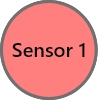
\includegraphics[width = 1 cm]{Grafik/Sensorelement.jpg} & ToDO\\
	\vspace{0cm}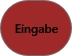
\includegraphics[width = 1 cm]{Grafik/Eingabe-Sensor.jpg} & ToDO\\
	\vspace{0cm}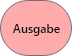
\includegraphics[width = 1 cm]{Grafik/Ausgabe-Sensor.jpg} & ToDO\\
	\vspace{0cm}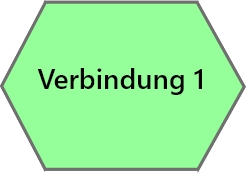
\includegraphics[width = 1 cm]{Grafik/Verbindungselement.jpg} & ToDO\\
	\vspace{0cm}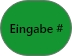
\includegraphics[width = 1 cm]{Grafik/Eingabe-Verbindung.jpg} & ToDO\\
	\vspace{0cm}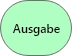
\includegraphics[width = 1 cm]{Grafik/Ausgabe-Verbindung.jpg} & ToDO\\
	\vspace{0cm}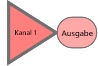
\includegraphics[width = 1 cm]{Grafik/Kanal.jpg} & ToDO\\
	\vspace{0cm}
\includegraphics[width = 1 cm]{Grafik/Verbindungspfeil.jpg} & ToDO\\
\end{tabular}

\subsection{Erweiterungsmöglichkeiten}

\section{Spezielle Anforderungen an die Entwicklungsumgebung}

\section{Zeit- und Ressourcenplanung}

\subsection{Projektphasen}

\begin{tabular}{| l | l | l | r |}
	\hline
	\textbf{Phase} & \textbf{Verantwortlicher} & \textbf{Zeitraum} & \textbf{Kolloquium} \\ \hline
	Pflichtenheft & Jan Küblbeck & KW 20–22 & 04.06.2019 \\
	Entwurf & Leon Huck & KW 23–26 & 02.07.2019 \\
	Implementierung & Stefan Geretschläger & KW 27–29, 31 & (?) \\
	Klausurenphase & — & KW 30, 32 & — \\
	Qualitätssicherung & David Gawron & KW 33–35 & 03.09.2019 \\
	Abnahme & — & KW 36 & — \\
	Abschlussprüfung & Linus Ruhnke & KW 37/38 & (?) \\
	\hline
\end{tabular}

\subsection{Entwurfsphase}

\subsection{Implementierungsphase}

\section{Ergänzungen}

\section{Glossar}

\renewcommand*{\glossarysection}[2][]{}	% prevents double glossary section heading
\printnoidxglossaries				% generate pdf twice when adding new entries


\end{document}